\clearpage

\chapter{\textbf{Resultados}}\label{results}
\section{Figura com subfiguras}\label{res:subfigure}
As in this case the figure with subfigures is quite big, it will appear in the next page. If they are smaller, they also fit within the text flow.\\
In the square brackets after 'begin figure' or 'begin subfigure, the command 'trim = l b r t' is cutting the figures on the left, bottom, right and top. Additionally, 'clip' is needed afterwards. 'rotate' can be used to rotate the figure. In the curly brackets the size of the figure can be adjusted either by using a defined width eg. 4~cm or by a percentage of the textwidth.
\begin{figure}[p]
    \centering % <-- added
\begin{subfigure}{0.75\textwidth}
  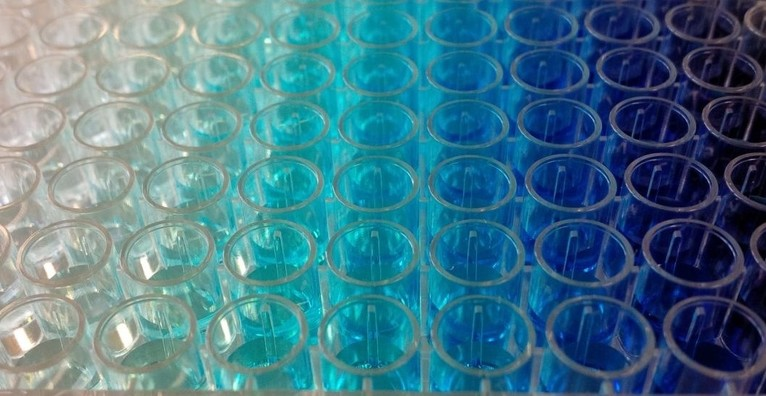
\includegraphics[trim = 30mm 15mm 0mm 20mm, clip,
  width=\linewidth]{pic/anyfigure.png}
  \caption{Caption for the first subfigure}
  \label{fig:1}
\end{subfigure}\hfil % <-- added
\begin{subfigure}{7 cm}
  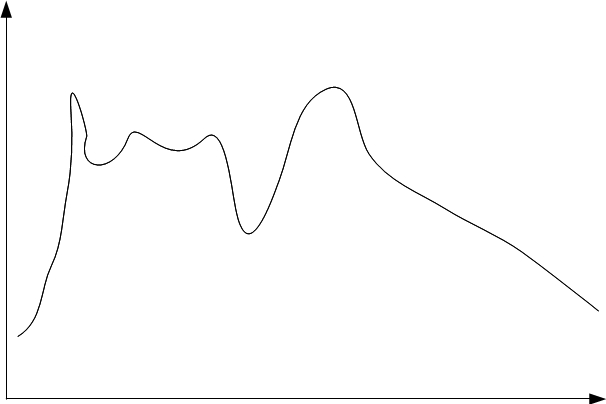
\includegraphics[trim = 30mm 15mm 0mm 20mm, clip, rotate=180, width=\linewidth]{pic/example.jpg}
  \caption{Caption for the second subfigure}
  \label{fig:2}
\end{subfigure}\hfil % <-- added

\medskip
\begin{subfigure}{0.75\textwidth}
  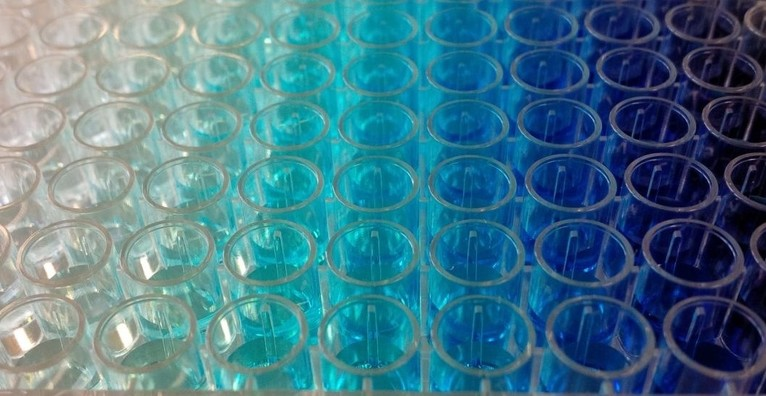
\includegraphics[trim = 30mm 15mm 0mm 20mm, clip, width=\linewidth]{pic/anyfigure.png}
  \caption{Caption for the third subfigure}
  \label{fig:3}
\end{subfigure}\hfil % <-- added

\caption[Figure with multiple subfigures]{3 subfigures can be combined in one figure. Each subfigure has a short caption and the figure itself has a caption underneath}
\label{fig:FACS-diff-comparison}
\end{figure}


\addtocontents{toc}{\vspace{0.8cm}}